\subsubsection{Página inicial do painel do docente}
\label{ssub:teacher_dashboard}

Esta página é dirigida aos docentes autenticados, e é a primeira página que estes consultam após o registo ou autenticação.

Tal como foi referido na secção ~\ref{ssub:student_dashboard}, esta é a primeira página consultada e deve conter as ações mais importantes para um docente.
Além da listagem dos vários tipos de projetos, tal como acontece com os alunos, um docente tem acesso rápido à criação de um projeto (figura ~\ref{fig:teacher_project_new}).

\begin{figure}[H]
  \centering
  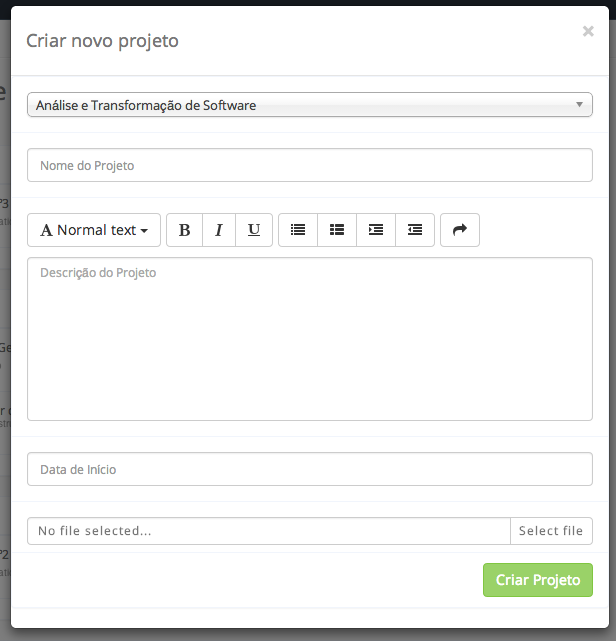
\includegraphics[width=1\textwidth,center]{images/implementacao/docentes/new_project}
  \caption{Novo projeto}
  \label{fig:teacher_project_new}
\end{figure}


Na Figura~\ref{fig:teacher_dashboard} pode ser consultada uma imagem demonstrativa da página desenvolvida.

\begin{figure}[H]
  \centering
  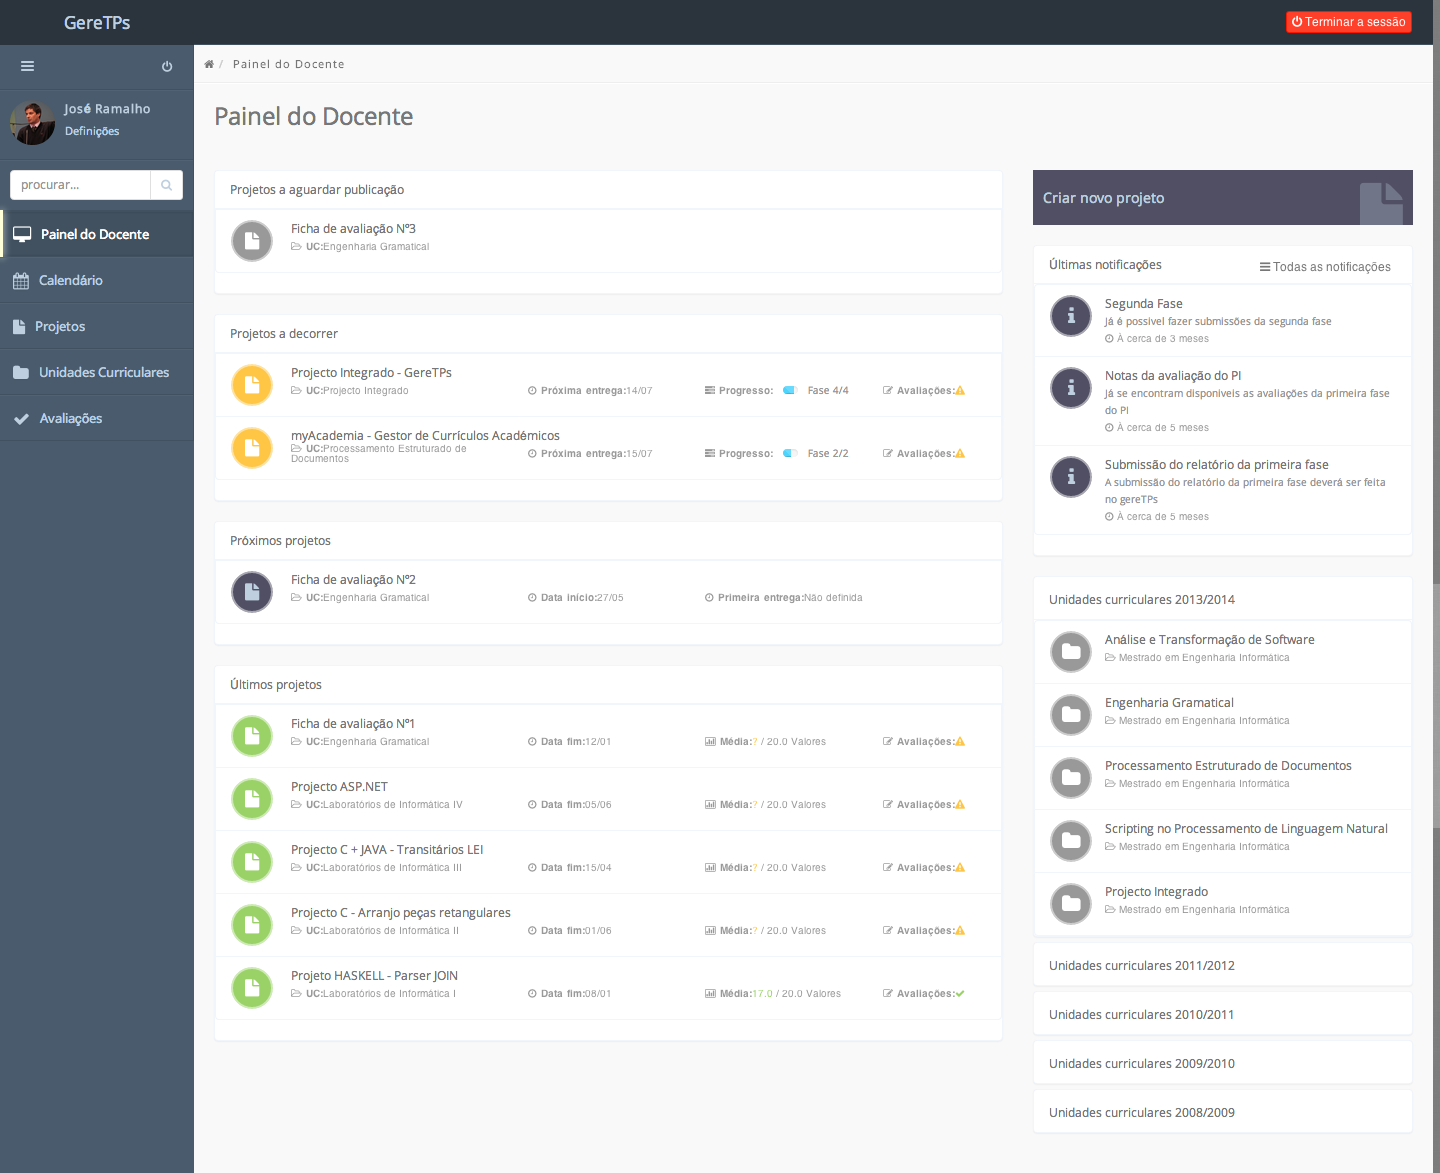
\includegraphics[width=1\textwidth,center]{images/implementacao/docentes/dashboard}
  \caption{Página inicial do painel do docente}
  \label{fig:teacher_dashboard}
\end{figure}
